\documentclass[conference]{IEEEtran}
\usepackage{cite}
\usepackage{amsmath,amssymb,amsfonts}
\usepackage{algorithmic}
\usepackage{graphicx}
\usepackage{textcomp}
\usepackage{xcolor}
\def\BibTeX{{\rm B\kern-.05em{\sc i\kern-.025em b}\kern-.08em
    T\kern-.1667em\lower.7ex\hbox{E}\kern-.125emX}}
\begin{document}

\title{Review Paper: Decision Transformer-Reinforcement Learning via Sequence 
Modeling}

\author{\IEEEauthorblockN{Sanjeev Kumar}
\IEEEauthorblockA{\textit{Institute for Data Science in Mechanical Engineering} \\
\textit{RWTH University}\\
Aachen, Germany \\
sanjeev.kumar@rwth-aachen.de}
}

\maketitle

\begin{abstract}
In Reinforcement Learning (RL), methods based on the Temporal Difference (TD) learning are commonly used to model agent behavior.  However, these methods can have an unstable objective function, making scaling difficult. To scale RL approaches to matured data-driven methods used in a domains like natural language processing (NLP) and Vision, we can view RL as a generic sequence modeling problem and leverage the existing high-capacity sequence prediction model architectures such as GPT-x and BERT. Viewing RL in this way offers stable learning and scalability, allowing the agent to learn wider policy distribution. This paper reviews the Decision Transformer (DT) \cite{b1}, a new RL approach based on Transformer architecture, which outputs the optimal future actions conditioned on the desired goal, i.e., return-to-go. Further, Chen et al.\cite{b1} demonstrate DT capabilities on Atari, OpenAI Gym, and key-to-door tasks and show that it performs comparably or better than other state-of-the-art model-free offline RL approaches.
\end{abstract}


\section{Introduction}
Sequential decision-making is one of the fundamental problems in artificial intelligence, for which researchers are using RL.
In the standard approach of RL, an agent learns while interacting with an environment. The agent observes the current state of the environment, based on it, takes action, and in return, receives a reward and the next state. The agent's primary goal is to maximize the cumulative reward over time.

These traditional approaches use TD learning to train a policy based on the TD error, which is the difference between the actual received reward and the predicted expected reward multiplied by the discount factor [2, pp. 143-144]. The discount factor (if high enough) can lead to short-sighted behavior in the agent, which is undesirable for long-term credit assignment tasks. An intuitive example of this in robotics is a robot learning to navigate in an environment to reach a destination. Suppose the robot is short-sighted and focuses more on immediate rewards for its action, such as moving forward. It may lead to sub-optimal policy, such as taking a longer path to receive a high immediate reward. Hence, a robot may fail to learn a good policy for navigation in the environment and not be able to reach the destination efficiently. 

However, in contrast to the traditional RL regime, RL can also be viewed as a sequence modeling problem. The wider distribution of an agent's behavior can be modeled using a Transformer architecture\cite{b3}. This architecture, which is currently a popular tool for capturing long-term dependencies, has been used in various domains, such as language and vision, and is effective in tasks such as text-to-image generation\cite{b4}, few-shot learning in language\cite{b5} and recent use case in ChatGPT. The key component of the Transformer architecture is the self-attention mechanism, which allows the model to focus on specific parts of the input sequence when generating the output. However, Transformer has been relatively unstudied in RL until\cite{b6}, where an architectural modification was proposed to improve its learning speed and stability in this setting. In many practical applications, such as training robots to perform specific tasks in a factory setting, offline RL\cite{b7}  holds great potential to turn large datasets into powerful decision-making engines. However, due to distribution shifts in offline RL, which refers to a change in the distribution of the environment's state transitions, rewards, or both, solving this problem can be complex, and prior algorithms have studied constraint policy action spaces\cite{b8} and incorporate value pessimism\cite{b9} to address this issue.

This review paper investigates\cite{b1}, and provides more insight into the usage of generative pretraining (GPT)\cite{b10} approach to process the input trajectory sequence of RL in auto-regressive manner. This means that the output is generated based on the previous tokens in the input sequence. Decision Transformer\cite{b1} approach that is being studied here is only applied to offline RL settings, where the agent is given a fixed set of past interactions to learn the policy, which is similar to fixed datasets that Transformers are traditionally trained with in NLP. 

\begin{figure}[htbp]
\centerline{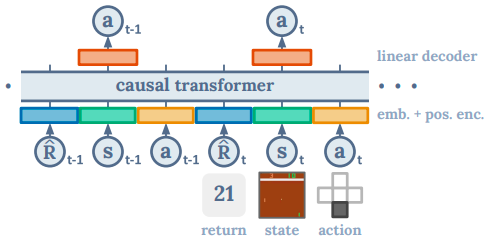
\includegraphics[scale=0.51]{Images/dt_intuition.png}}
\caption{Decision Transformer architecture. States, actions and returns-to-go are fed into the linear embeddings and positional episodic time-step encoding is added. Tokens are fed into a GPT architecture to
predicts actions autoregressively using a casual self-attention
mask\cite{b1}.}
\label{fig}
\end{figure}

\section{PRELIMINARIES}
This section covers the foundational concepts of offline RL, autoregressive models, and Transformer, which are necessary to comprehend the reviewed paper.

\subsection{Offline Vs Online Reinforcement Learning}
Online RL is sub-field of machine learning that modeled the environment in a Markov Decision process (MDP) framework denoted in form of tuple \( \langle S, A, P, R \rangle\), where \(S\) is a state space, \(A\) is a action space, \(P(s_{t+1} | s_t, a_t)\) is the state transition probability, and \(R (s_t, a_t)\) is the reward function. At each time step agent observes a state \( s_t \in S\) and takes an action \( a_t \in A\) and transition to next state \( s_{t+1} \in P(.|s_t, a_t)\). In each transition agent receives a reward \( r_t = R(s_t,a_t)\). The agent's goal is to maximize the expected cumulative reward. Online RL is characterized by real-time learning as the agent adapts to changing dynamics in the environment, and can use on-policy or off-policy methods for learning.

However, Offline RL \cite{b7} utilizes a fixed interaction dataset collected by arbitrary policies, as illustrates in Fig. 2. The agent's behavior is not adaptable to the environment like online RL. However, while learning offline, the agent can still use the on-policy or off-policy method. This approach closely resembles standard supervised learning.


\subsection{Autoregressive Models}\label{AA}

Autoregressive models are a feed-forward model which predicts the next variable in a sequence based  on the past variables, for instance the \( k^{th}\) order autoregressive model predicts the next variable \(x_t\) in the sequence based on the \( k\) previous variables \( (x_{t-1}, x_{t-2},..., x_{t-k})\).
\begin{equation}
x_t = f(x_{t-1}, x_{t-2},....., x_{t-k}).
\end{equation}


These models make a strong conditional independence assumption. The same concept can be extended to situations with different inputs and outputs for instance language translation. One way to enhance the performance of autoregressive models is by incorporating the self-attention mechanism of transformer architecture. This creates a new type of model called an Autoregressive Transformer, which can make predictions by assigning varying importance to different tokens in the input sequence. 



\begin{figure}[htbp]
\centerline{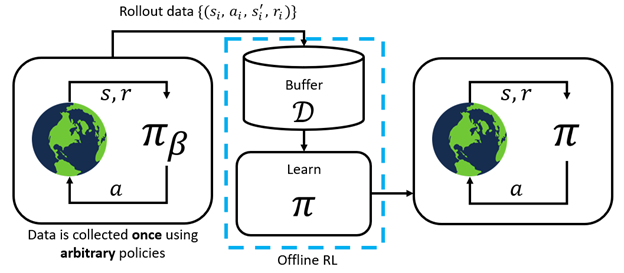
\includegraphics[scale=0.39]{Images/offlineRL.png}}
\caption{Illustration of offline RL, where a datatset D collected by some(potentially unknown) behavior policy \(\pi_{\beta}\). The dataset is collected once, and is not altered during training, which makes it feasible to use large previous collected datasets. The training process does not interact with the MDP at all, and the policy is only deployed after being fully trained \cite{b7}.}
\label{fig}
\end{figure}


\subsection{Transformer}\label{AA}
This subsection delves into the intricacies of the Transformer model [3] by closely examining its components. The Transformer follows the common encoder-decoder structure of most neural machine translation models, as seen in Fig. 3. The Encoder part (shown on left side) maps
an input sequence \((x_1, x_2, .., x_n)\) to a sequence of the continuous hidden representation \(\textbf{z} = (z_1, z_2, .., z_n)\). The Decoder part (shown on right side) uses \textbf{z} to produce an output sequence
\((y_1, y_2,.., y_n)\) one at a time. Transformer is auto-regressive
model in nature, hence considering the previously predicted
output as additional input when generating the output for the next
time step. This simple network architecture is entirely based on
a memory mechanism called self-attention.

\paragraph{\textbf{Attention vs Self-Attention}}
The memory network that focuses on different elements of the input sequence for output prediction  is called attention. Two similar words are used in literature of the neural models, attention
and self-attention. Both are similar in working, allow a model
to focus on different parts of the input when processing it.
There is one key difference between both, attention mechanism
are used in neural machine translation, where model needs to
focus on different parts of the source sentence when generating
the target sentence.

\begin{figure}[htbp]
\centerline{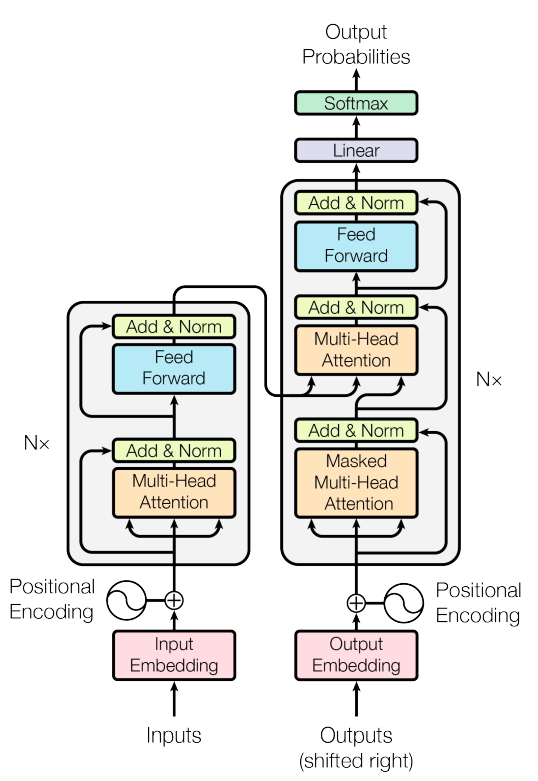
\includegraphics[scale=0.37]{Images/architecture.png}}
\caption{Transformer architecture. Inputs are fed into linear embedding and a positional encoding is added, which fed into encoder block (left). Output embedding are offset by one position, before fed into decoder block (right), ensures that the predictions for position \(i\) can depend only on the known outputs at position less than \(i\)\cite{b3}.}
\label{fig}
\end{figure}


However, self-attention is a specific type of attention mechanism that allows a model to focus on different parts of the input sequence within the same model. The attention is self-contained within the model architecture, which means the model does not need any external information to compute the attention weights. 
\paragraph{\textbf{Scaled Dot-Product Attention}}
The key to the success of the Transformer in the NLP application, such as ChatGPT and vision task, is the scaled dot-product attention mechanism, as shown in Fig. 4. In the Transformer architecture, input tokens are represented as embeddings in a continuous vector space. These embeddings undergo multiple linear projections to create \textit{queries} and \textit{keys} of dimension \(d_k\) and \textit{values} of dimension \(d_v\). The attention values depicted in \eqref{eq:2} reflect the similarity between the query token and every other token in the sequence and are determined by taking the dot product between the query and all the keys, which is then scaled down (divided by \(\sqrt{d_k}\)) and passed through a softmax function. The new contextualized embeddings are created by computing the weighted sum of the \textit{values}. The weights assigned to each \textit{value} are the \textit{attention value} computed by the scalar dot-product between the query and the corresponding key.
In practice, the attention function simultaneously computes the set of queries packed together in matrix \(Q\). Similarly, keys and values are packed together in K and V matrices and output attention matrix as \cite{b3}:

\begin{equation}\label{eq:2}
\mathrm{Attention} \((Q,K,V) = {{{\underbrace{\mathrm{softmax}\left( \frac{QK^T}{\sqrt{d_k}} \right )}_{\text{attention values}}} V.} }\)
\end{equation}

In Transformer, instead of single-head attention, multi-head attention is used. Multi-head attention allows the model to be more parallelizable. Each attention head is focused on a different input part and can learn to focus on different types of information. This allows the model to be more expressive and handle a variety of tasks \cite{b3}.

\begin{equation}
\mathrm{MultiHead}\((Q,K,V) = \mathrm{Concat}(head_1,..,head_h)W^O.\)
\end{equation}

where \( \mathrm{head_i} = \mathrm{Attention}(QW_i^Q, KW_i^K, VW_i^V).\)
\\


\begin{figure}[htbp]
\centerline{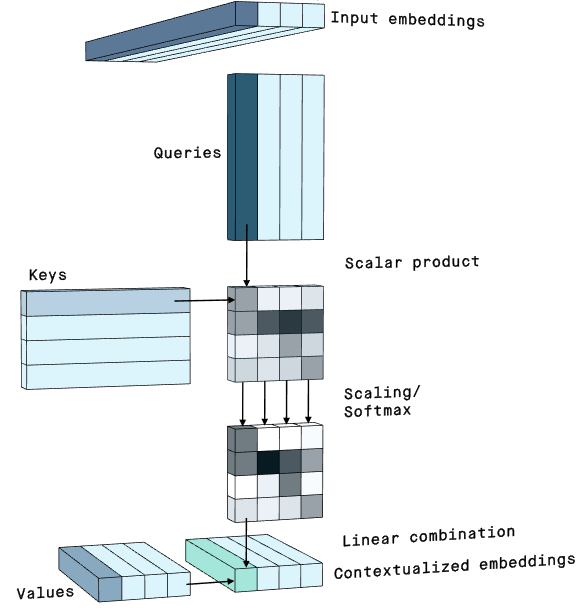
\includegraphics[scale=0.4]{Images/scaled_dot_product.png}}
\caption{Illustration of Scaled Dot-Product Attention. Input embeddings are converted into queries, keys and values matrices. The scalar products between a query and the keys, which give the level of relationship between the query’s token and every other token, are typically scaled down for numerical stability, then passed through a softmax activation function. The new contextualized embeddings are created by combining the values corresponding to every input token, in proportions given by the results of the softmax function\cite{b11}}
\label{fig}
\end{figure}

\paragraph{\textbf{Encoder}}
The Encoder block in Transformer architecture comprises a stack of N identical layers (that do not share any weights), as shown in Fig. 3. Further, each layer is broken down into two sub-layers. The first sub-layer is a  multi-head self-attention mechanism that takes embedding representations of sequence as input in the form of query, key, and value vector. The output of the multi-head self-attention is fed to the feed-forward neural network. Each sub-layer (multi-head self-attention, FFNN) in each encoder layer has a residual connection around it and is followed by a layer-normalization step.
\paragraph{\textbf{Decoder}}
The Decoder block in Transformer architecture also comprises a stack of N identical layers. In respect to the encoder block, the decoder block contains third sub-layer in addition to two sub-layers of the encoder part. The third sub-layer took the output of the encoder block and transformed it into key and value matrices. The multi-head self-attention sub-layer uses both of these, which also takes the query matrix from the layer below it. The self-attention mechanism in the bottom decoder layer works slightly differently than in the upper decoder. It is only allowed to attend to earlier positions in the output sequence. This is done by masking future positions (setting them to \(\infty\)) before the softmax step in the scaled dot-product step. This masking, combined with the fact that output embeddings are offset by one position, ensures that predictions for position \(i\) can only depend on the known output at positions less than \(i\)\cite{b3}. Like the encoder, each sub-layers has residual connections around it, followed by layer normalization.

\subsection{Generative Pre-Training (GPT)}\label{AA}
In the field of NLP, there is a growing effort to leverage large amounts of raw data to reduce dependency on supervised learning. One such method is generative pre-training \cite{b10}, which is a semi-supervised approach based on Transformer architecture\cite{b3}. Self-supervised learning is a method where the model is trained using a combination of unsupervised pre-training and supervised fine-tuning. For pre-training, we have raw input data that does not have explicit labels. Instead, the labels are computed from the input data itself. For example, if we have a book containing roughly 10,000 words, and we want to predict the next word in a sentence based on the sequence of the previous word (101st word based on the previous sequence of 100 words). For this, we can create a large training set by sliding a window of size 100 over the whole book. The main idea of GPT is to use pre-training as a first step to learn universal representations of the raw input data, which can then be fine-tuned in the second step for a specific task using a smaller labeled dataset. The pre-training step is typically done on unlabeled data using the language modeling objective, which is to maximize the following likelihood given an unsupervised corpus of tokens \( U = \{u_1,...,u_n\}\)\cite{b10}.

\begin{equation}
L_1(U) = \sum_{i} \log P(u_i|u_{i-k},..,u_{i-1}; \theta),
\end{equation}
where k is the size of the context window (512), and the conditional probability \(P\) is modeled using a neural network with parameters \(\theta\), which will be trained using stochastic gradient descent.



In GPT, the initially proposed Transformer architecture has been modified. The model only used the decoder block of the Transformer with 12 layers, depicted in Fig. 5. In\cite{b10}, Alec et al. specify a context length of 512 for training the model. The context length parameter determines the number of previous tokens (words/phrases/characters) the model will consider when making the next prediction. For example, consider the sentence, ''The cat sat on the mat.'' If a model has a context length of 2, it will consider the previous two words, "sat on," to understand the semantic and predicts the next word, "the." Since the Transformer-based model takes the whole sequence as input in contrast to RNN methods. In self-attention mechanisms, the  "masking" technique prevents the model from peeking into the future when making predictions and is implemented by setting the attention weights corresponding to future tokens to zero; thus, the Transformer used in GPT is known as a Causal Transformer.


\begin{figure}[htbp]
\centerline{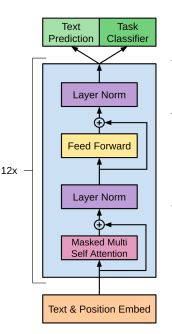
\includegraphics[scale=0.5]{Images/gpt_architecture.png}}
\caption{GPT Model Architecture, based on Transformer decoder block which has 12 layers\cite{b10}.}
\label{fig}
\end{figure}


\section{Decision Transformer Methodology}
\subsection{Motivation}
The paper [1] presents a new framework for reinforcement
learning called Decision Transformer (DT). The primary motivation
to introduce this framework in RL is to utilize the Transformer
architecture’s ability to handle sequential data, which enables it
to effectively model the dependencies between actions and
observations from the large available corpus of data. The pre-training
step of the GPT \cite{b10} allows to learn general representations
of the input data (logged set of agent’s interactions), which
further can be fine-tuned for specific decision-making tasks via
incorporating online interactions of the agent with the environment,
resulting in more sample-efficient online RL for downstream
tasks. As DT work is an initial attempt in this direction and lacks the fine-tuning step of policies trained on offline data. An added advantage of this framework is that,
DT does not require policy regularization or conservatism (technique to prevent agent for taking actions that are too risky)
to mitigate the overfitting to the training data in offline RL
to achieve good performance. Additionally, the attention
mechanism in the Decision Transformer can be used to handle
partial observability in the RL problem.

\subsection{Trajectory Representation}
In MDP framework trajectory sequence of RL is represented as \((s_1, a_1,..,s_T,a_T)\), where next state is conditioned to previous state and action as shown in Fig. 6(a). The limitation of this graphical 
 model is that it doesn’t tell how to choose the optimal action in the state.  To enable the current RL regime to conditionally generate the action in current state based on future desired return \eqref{eq:5c}, rather than maximizing the cumulative reward,  Chen et al.\cite{b1} introduced optimality variable inspired by the work\cite{b12}. They encoded this optimality variable as return-to-go (RTG) as shown in Fig. 6(b). Let \(\mathcal{T}\) denote the trajectory sequence upto time step \(T\). The RTG at timestep \(t\), \(R_{t} = \sum_{t'=t}^{T} r_{t'}\), is the sum of future rewards from that
timestep. This leads to modified trajectory representation consist of: RTGs, states and actions \(\mathcal{T}= (R_{1},s_{1},a_1,R_2,s_2,a_2,...,R_T,s_T,a_T) \), which is amenable to autoregressive training and generation via GPT architecture.

\begin{subequations}\label{eq:5}
\begin{align}
  p(O_t|s_t,a_t)& \propto p(a_t|s_t,O_t).\label{eq:5a} &\text{Bayes' Rule} \\
                & \Rightarrow \p(a_t|s_t,R_t).\label{eq:5b} &\text{Markovian env.} \\
 & \Rightarrow \p(a_t|s_t,R_t,a_{t-1},R_{t-1},...).\label{eq:5c} &\text{Non-Markovian env.}
\end{align}
\end{subequations}
\begin{figure}[htbp]
\centerline{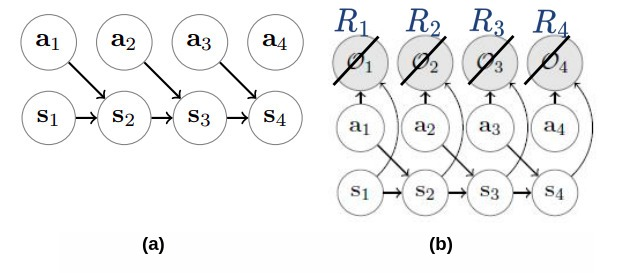
\includegraphics[scale=0.35]{Images/graphical_model.jpg}}
\caption{(a) graphical model of MDP, next state conditioned on previous state and action. (b) In order to embed conditional inference in RL i.e condition on optimality variable: RTG being true, generate most probable action sequence.\cite{b12}.}
\label{fig}
\end{figure}

\subsection{Architecture}\label{AA}
Like GPT, the Decision Transformer uses the decoder part of the Transformer architecture. It processes a trajectory \(\mathcal{T}= (R_{1},s_{1},a_1,R_2,s_2,a_2,...,R_T,s_T,a_T) \) as a sequence of 3 types of input tokens: RTGs, states, actions, which is distinct from how a token is used in NLP tasks. For example, when feeding a trajectory of K time-steps to DT, the input is 3K tokens. At timestep \(t\), DT uses the tokens from the last K timesteps to predict an action \(a_t\). Here, K is the hyperparameter, referred to as context length for the Transformer. This is illustrated in Fig. 1, where the prediction of \(a_t\) is conditioned on everything that came at time-step \(t-1\) and also return-to-go and state at time-step \(t\). In addition, there is a key difference in positional encoding between DT and Transformer. In a standard Transformer, the learnable positional encoding is typically added to the input embeddings before they are passed through the Transformer layers depicted in Fig. 3. Since Transformer takes a complete sequence as input to allow the  model to distinguish between different positions, positional encoding vectors are chosen such that they are unique for each position in the sequence. In DT the positional encoding is slightly different, as the inputs are sequences from RL trajectories, which consist of return-to-go, state, and action tokens at each time step. The positional encoding in DT is used to provide the model with information about the position of each input in the sequence, but also the information about the type of input (return-to-go, state, action) that the model is processing at each time step.

\paragraph{\textbf{Forward pass}}
In the Decision Transformer input is given in the form of a sequence of states, actions, and a term known as returns-to-go (RTGs): \((R_{1},s_{1},a_1,R_2,s_2,a_2,...,R_T,s_T,a_T)\). DT learns a deterministic policy
\(\pi_{DT}(a_t|R_{t-1},s_{t-1},..,R{t-k},s_{t-k})\), parameterized by GPT architecture\cite{b10} and outputs the optimal action at each state, using Autoregressive Casual Transformer, to achieve the set target return. The self-attention mechanism of the Transformer decides which past actions are more important to consider when predicting the action in the current time step. The self-attention is computed over a context length K. The Decision Transformer is trained to predict actions by utilizing either cross-entropy loss for discrete actions or mean-squared error for continuous actions, which are easy to optimize and helps to scale the RL problem.

\paragraph{\textbf{Rollouts: How to use the DT model}}
The sequence of actions is generated in a autoregressive way i.e. using the predicted output as input for the next prediction. To evaluate the DT model, two quantities are required: the desired performance \(R_1\) and the initial state \(s_1\). DT generates the action \(a_1=\pi_{DT}(R_1,s_1)\), which agent executes on the current state \(s_1\) to collect reward \(r_1\) and transitioned in new state \(s_2\). For the next action \(a_2\), new RTG is computed as \(R_2 = R_1 - r_1\) and DT generates \(a_2\) based on \((R_2,s_2,R_1,s_1)\) as : \(a_1 = \pi_{DT}(R_2,s_2,R_1,s_1)\). This process is repeated until the end of episode.

\section{Experiments and Results}This section assesses the effectiveness of DT by comparing its results to other offline RL and imitation learning baselines. DT is compared to model-free offline RL algorithms based on TD learning because it is a model-free method, and TD learning is widely used for sample efficiency in current RL literature. The comparison with imitation learning algorithms is due to their similar likelihood-based policy learning approach to DT. The performance of the
model is evaluated by analyzing the return it produces.
\subsection{Environment description and setup}
The presented DT framework is evaluated on the offline RL benchmarks in Atari\cite{b13}, Open AI Gym\cite{b14}, and Key-to-Door\cite{b15} environment.
\paragraph{\textbf{Atari}}
The Atari benchmark is a collection of Atari 2600 games used for quite a while as a benchmark in RL research to evaluate the effectiveness of reinforcement learning algorithms for discrete control tasks. These games are challenging for RL algorithms due to their large state spaces, hard-to-predict dynamics, and infrequent rewards. Chen et al.\cite{b1} have compared DT performance to other baselines on four Atari tasks: Breakout, Q*bert, Pong, and Seaquest, and used the 1\% of all samples in DQN-replay dataset presented in \cite{b16}.
\paragraph{\textbf{OpenAI Gym}}
OpenAI Gym provides a standardized environment for evaluating the performance of different RL algorithms developed for continuous control tasks. Chen et al.\cite{b1} have used the D4RL benchmark\cite{b17}, which includes environments such as HalfCheetah, Hopper, and Walker, to test the performance of DT. Since DT is designed for offline RL, the dataset settings used to collect the data are important, and different settings such as Medium, Medium-Relay, and Medium-Expert were used.

\paragraph{\textbf{Key-to-Door}}
To test DT's ability to assign credit over a long period, the variant of the Key-to-Door environment proposed in\cite{b15} is used. This environment is grid-based and has 3 phases. In the first phase, the agent is placed in a room with a key. In the second phase, the agent is placed in an empty room, and in the third phase, the agent is put in a room with a door. The agent only receives a binary reward when it opens the door in the third phase if it had picked up the key in the first phase. This task is challenging for credit assignment because the credit must be distributed over the entire episode, including actions taken in the second phase.

\begin{figure*}
  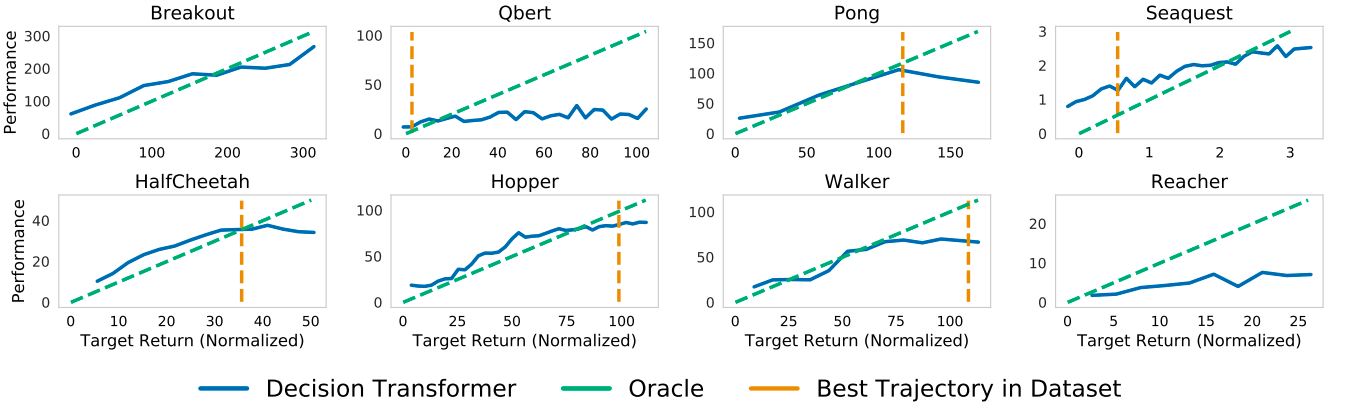
\includegraphics[width=\textwidth, height=4.7cm]{Images/result.png}
  \caption{Sampled (evaluation) returns accumulated by Decision Transformer when conditioned on the specified target (desired) returns. \textbf{Top}: Atari, \textbf{Bottom}: D4RL medium-replay datasets\cite{b1}.}
\end{figure*}
\subsection{Experimental Evaluation Results}

Chen et al.\cite{b1} have compared the performance of DT to other algorithms such as CQL\cite{b18}, REM\cite{b16}, and QR-DQN\cite{b19} on Atari tasks, and CQL\cite{b18}, BEAR\cite{b20}, BRAC\cite{b21}, and AWR\cite{b22} on OpenAI gym tasks. They also include results for Behavior Cloning (BC), which has the same network architecture and hyperparameters as DT but does not include return-to-go conditioning. The performance of DT in all scenarios is summarized in Fig. 8, where performance is represented as a normalized episode return.


\section{Discussion}
This review paper covers the first research work on using the Transformer architecture for sequence modeling in RL and outlines the DT methodology. Transformer-based models are well-known for modeling large distributions of variables. Chen et al.\cite{b1} also evaluated how well DT models the distribution of returns. They did this by varying the desired target return and evaluating DT's understanding of the RTG token. Fig. 7 shows the results of return conditioning and demonstrates that by varying the notion of the target return, it is possible to achieve multi-tasking in some sense. For example, if the desired target return for a hopper is low, it will remain stationary. However, if it is high, the hopper will move forward by hopping. In Fig. 7, the x-axis represents the normalized desired target return, and the y-axis shows the return achieved from DT. The green line, or "oracle," represents the ideal scenario where the model is perfect, and we get whatever we desire from DT. In DT, since interaction data is collected offline, the orange line represents the trajectory with the greatest return in the dataset. For most environments, there is a good match between the desired target return and the actual achieved return. In tasks like Pong, HalfCheetah, 
\begin{figure}[htbp]
\centerline{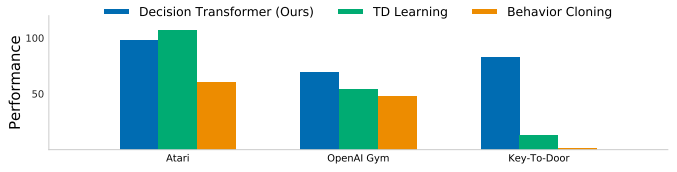
\includegraphics[scale=0.4]{Images/result_2.png}}
\caption{Results comparing DT to TD learning(CQL) and behavior cloning across Atari, OpenAI Gym, and Minigrid. On a diverse set of tasks, DT performs comparably or better than traditional approaches\cite{b1}.}
\label{fig}
\end{figure}
and Hopper, DT generates trajectories that almost perfectly match the desired returns. However, in some cases, like in the Seaquest task, DT extrapolates. In Seaquest, the highest return trajectory in offline data is relatively low, but the model is still able to generate a trajectory that achieves a higher return. 

The original paper\cite{b1} extensively examines the capabilities of the DT model by discussing various experiments, such as the ability to effectively handle long credit assignments, which traditional TD learning approaches struggle with. The study specifically demonstrates the DT's ability to learn effective policies that lead to nearly optimal paths in the Key-to-Door environment. Additionally, the paper also investigates whether the DT can be used effectively as a critic by modifying it to output return tokens in addition to action tokens in the Key-to-Door environment. As opposed to regular DT, in this setting, the first return token is predicted rather than provided as input. The experiment shows that when the agent picks the key in the first phase and opens the door in the third phase, it receives the maximum return, whereas if it fails to pick the key in the first phase, it receives very low return.
\section{Summary}
The proposed DT work tried to bridge the gap between traditional RL techniques and data-driven methods used in NLP and Vision. The initial study provided strong evidence that treating RL as a sequence modeling problem can lead to similar or better performance compared to offline RL methods based on TD-learning. However, it is not yet possible to fully replace traditional RL methods with Transformer-based methods. The study also showed promising performance on various benchmarks, but the effectiveness of policies learned through offline RL is limited by the quality of the training dataset and further research is needed to incorporate online components for fine-tuning. Additionally, specifying the target return may be necessary to solve the RL task in DT, which is a pit-fall of this method. Transformer-based RL models can also be used to model the state evolution of trajectories, potentially serving as an alternative to model-based RL.

\begin{thebibliography}{00}
\bibitem{b1} L. Chen et al., ‘Decision transformer: Reinforcement learning via sequence modeling’,
Advances in neural information processing systems, vol. 34, pp. 15084–15097, 2021.
\bibitem{b2} Richard S Sutton and Andrew G Barto. Reinforcement learning: An introduction. MIT Press, 2018
\bibitem{b3}A. Vaswani et al., ‘Attention is all you need’, Advances in neural information processing
systems, vol. 30, 2017.
\bibitem{b4} A. Ramesh et al., ‘Zero-shot text-to-image generation’, in International Conference on Machine Learning, 2021, pp. 8821–8831.
\bibitem{b5} T. Brown et al., ‘Language models are few-shot learners’, Advances in neural information
processing systems, vol. 33, pp. 1877–1901, 2020.
\bibitem{b6} E. Parisotto et al., ‘Stabilizing transformers for reinforcement learning’, in International conference on machine learning, 2020, pp. 7487–7498.
\bibitem{b7}S. Levine, A. Kumar, G. Tucker, and J. Fu, ‘Offline reinforcement learning: Tutorial, review, and perspectives on open problems’, arXiv preprint arXiv:2005. 01643, 2020
\bibitem{b8} S. Fujimoto, D. Meger, and D. Precup, ‘Off-policy deep reinforcement learning without
exploration’, in International conference on machine learning, 2019, pp. 2052–2062.
\bibitem{b9}R. Kidambi, A. Rajeswaran, P. Netrapalli, and T. Joachims, ‘Morel: Model-based offline
reinforcement learning’, Advances in neural information processing systems, vol. 33, pp.
21810–21823, 2020.
\bibitem{b10} A. Radford, K. Narasimhan, T. Salimans, I. Sutskever, and Others, ‘Improving language
understanding by generative pre-training’, 2018.
\bibitem{b11} Romain Futrzynski, "Getting meaning from text: self-attention step-by-step video". peltarion.com. https://peltarion.com/blog/data-science/self-attention-video (accessed January 16, 2023)
\bibitem{b12} S. Levine, ‘Reinforcement learning and control as probabilistic inference: Tutorial and review’, arXiv preprint arXiv:1805. 00909, 2018.
\bibitem{b13}M. G. Bellemare, Y. Naddaf, J. Veness, and M. Bowling, ‘The arcade learning environment: An evaluation platform for general agents’, Journal of Artificial Intelligence Research, vol. 47, pp.
253–279, 2013.
\bibitem{b14}G. Brockman et al., ‘Openai gym’, arXiv preprint arXiv:1606. 01540, 2016.
\bibitem{b15}TT. Mesnard et al., ‘Counterfactual credit assignment in model-free reinforcement learning’,
arXiv preprint arXiv:2011. 09464, 2020.
\bibitem{b16}R. Agarwal, D. Schuurmans, and M. Norouzi, ‘An optimistic perspective on offline
reinforcement learning’, in International Conference on Machine Learning, 2020, pp. 104–114.
\bibitem{b17}J. Fu, A. Kumar, O. Nachum, G. Tucker, and S. Levine, ‘D4rl: Datasets for deep data-driven
reinforcement learning’, arXiv preprint arXiv:2004. 07219, 2020
\bibitem{b18}A. Kumar, A. Zhou, G. Tucker, and S. Levine, ‘Conservative q-learning for offline
reinforcement learning’, Advances in Neural Information Processing Systems, vol. 33, pp.
1179–1191, 2020.
\bibitem{b19} W. Dabney, M. Rowland, M. Bellemare, and R. Munos, ‘Distributional reinforcement learning
with quantile regression’, in Proceedings of the AAAI Conference on Artificial Intelligence,
2018, vol. 32.
\bibitem{b20}A. Kumar, J. Fu, M. Soh, G. Tucker, and S. Levine, ‘Stabilizing off-policy q-learning via
bootstrapping error reduction’, Advances in Neural Information Processing Systems, vol. 32,
2019.
\bibitem{b21}Y. Wu, G. Tucker, and O. Nachum, ‘Behavior regularized offline reinforcement learning’, arXiv
preprint arXiv:1911. 11361, 2019.
\bibitem{b22} X. B. Peng, A. Kumar, G. Zhang, and S. Levine, ‘Advantage-weighted regression: Simple and
scalable off-policy reinforcement learning’, arXiv preprint arXiv:1910. 00177, 2019.
\end{thebibliography}
\end{document}